\documentclass[11pt,letterpaper]{article}
\usepackage[lmargin=1in,rmargin=1in,tmargin=1in,bmargin=1in]{geometry}
\usepackage{../style/homework}
\usepackage{../style/commands}
\setbool{quotetype}{true} % True: Side; False: Under
\setbool{hideans}{true} % Student: True; Instructor: False

\newcommand{\blank}[1]{\underline{\hspace{#1}}} % Blank Underline

% -------------------
% Content
% -------------------
\begin{document}

\homework{18: Due 12/12}{It has been said that geometry is the art of applying good reasoning to bad diagrams.}{Richard J. Trudeau}

% Problem 1
\problem{10} Consider the graph $G$ shown below.
	\begin{figure}[h]
	\centering
	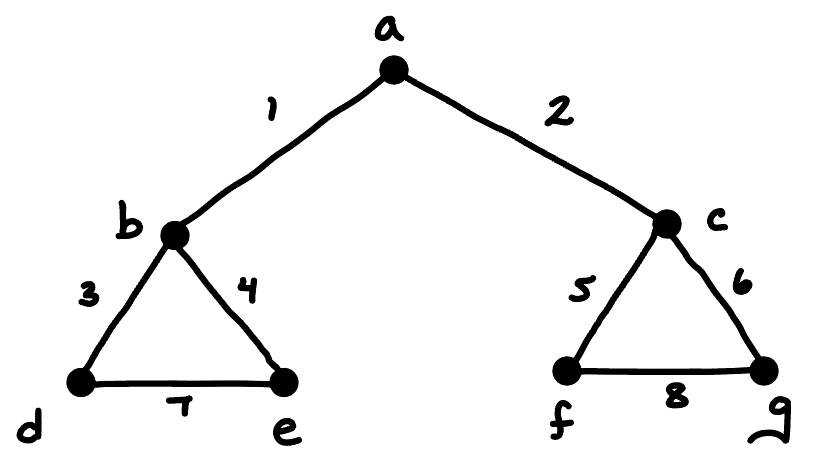
\includegraphics[width=0.35\textwidth]{graph1.jpg}
	\end{figure}

\begin{enumerate}[(a)]
\item Is the graph $G$ connected? Explain.
\item Is $d7e4b1a2c5f8g$ a trail? Explain. Is it a path? Explain.
\item Is $c5f8g6c2a$ a path? Explain. Is this walk closed? Explain.
\item Does this graph have a circuit? Explain. 
\item Let $A_G$ denote the adjacency matrix of $G$. Given the following:
	\[
	A_G^{10}=
	\begin{pmatrix}
	860 & 746 & 746 & 681 & 681 & 681 & 681 \\
	746 & 1282 & 940 & 884 & 884 & 543 & 543 \\
	746 & 940 & 1282 & 543 & 543 & 884 & 884 \\
	681 & 884 & 543 & 743 & 742 & 401 & 401 \\
	681 & 884 & 543 & 742 & 743 & 401 & 401 \\
	681 & 543 & 884 & 401 & 401 & 743 & 742 \\
	681 & 543 & 884 & 401 & 401 & 742 & 743
	\end{pmatrix}
	\]
How many closed walks are there starting at $a$? Explain. 
\end{enumerate}



\newpage



% Problem 2
\problem{10} Consider the graph $G$ shown below.
	\begin{figure}[h]
	\centering
	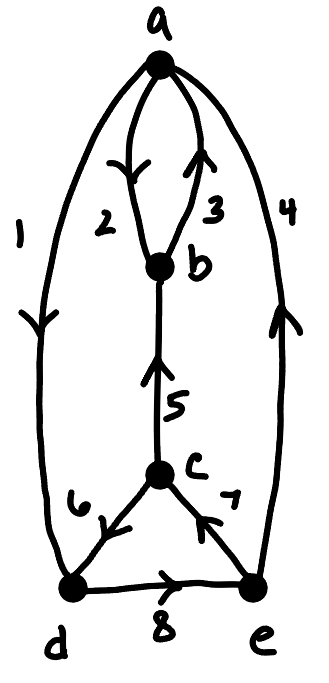
\includegraphics[width=0.14\textwidth]{graph2.jpg}
	\end{figure}

\begin{enumerate}[(a)]
\item Does there exist a Hamiltonian circuit for this graph? Explain. 
\item Does there exist an Euler circuit for this graph? Explain. 
\item Find the adjacency matrix for this graph.
\item Find the number of walks from $a$ to $b$ of length 4. Be sure to justify your answer. 
\end{enumerate}



\newpage



% Problem 3
\problem{10} Consider the graph $G$ shown below.
	\begin{figure}[h]
	\centering
	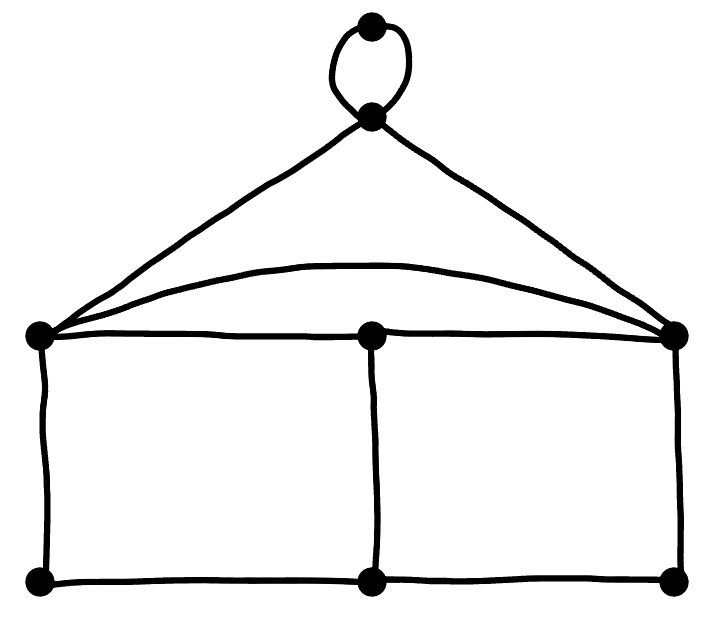
\includegraphics[width=0.3\textwidth]{graph3.jpg}
	\end{figure}

\begin{enumerate}[(a)]
\item Does there exist an Euler trail for this graph? If so, find one. If not, explain why.
\item Does there exist an Euler circuit for this graph? If so, find one. If not, explain why. 
\item Does there exist a Hamiltonian circuit for this graph? If so, find one. If not, explain why. 
\end{enumerate}



\newpage



% Problem 4
\problem{10} Showing all your work and fully justifying your reasoning, respond to the following:
	\begin{enumerate}[(a)]
	\item Does there exist a tree with 2023 vertices and 2024 edges? Explain. 
	\item Does a graph with five vertices and four edges have to be a tree? Explain.
	\item Find two non-isomorphic trees with five vertices. Be sure to explain why they cannot be isomorphic. 
	\end{enumerate}


\end{document}